\section{Implementation and Optimization}
\label{sec:pytheas:impl}



\begin{figure*}[t!]
\captionsetup[subfigure]{justification=centering,farskip=-1pt,captionskip=5pt}
\centering
%\hspace{-0.5cm}
\subfloat[API to application sessions]
{
        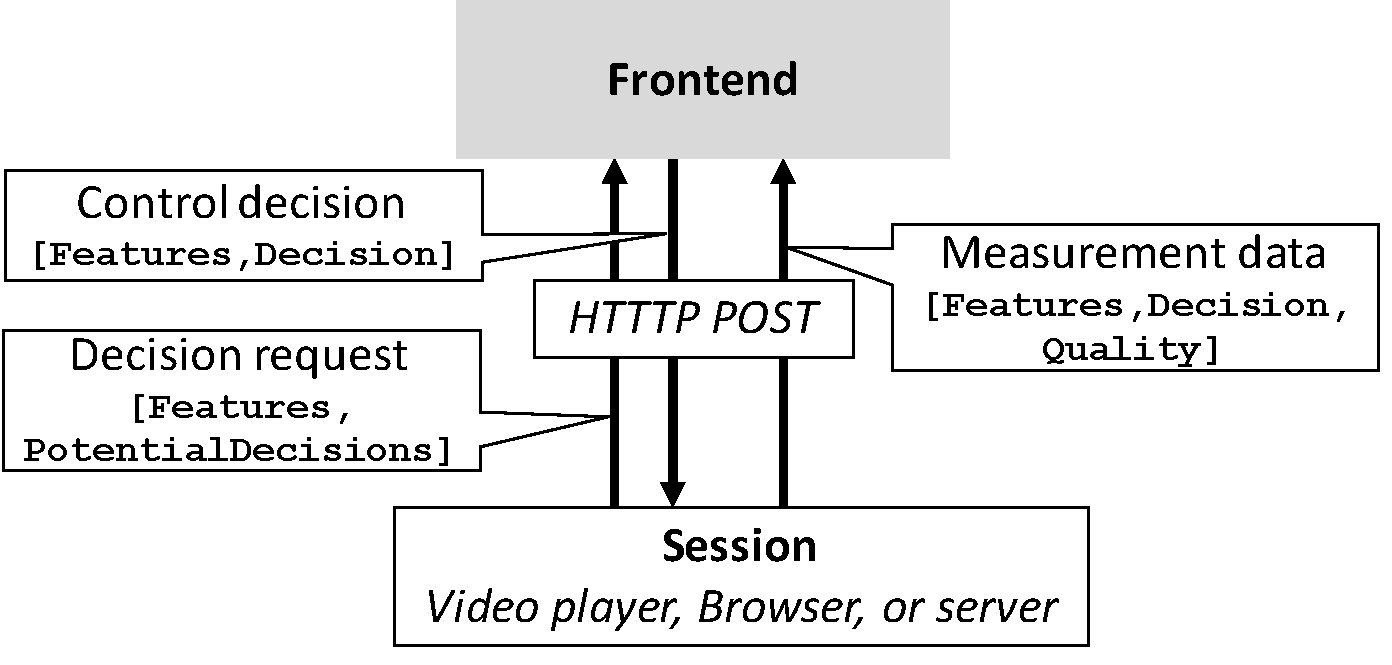
\includegraphics[width=0.6\textwidth]{figures/pytheas-impl-sep-api.pdf}
	\label{fig:impl-api}
}\\
%\hspace{-0.2cm}
\subfloat[Frontend]
{
        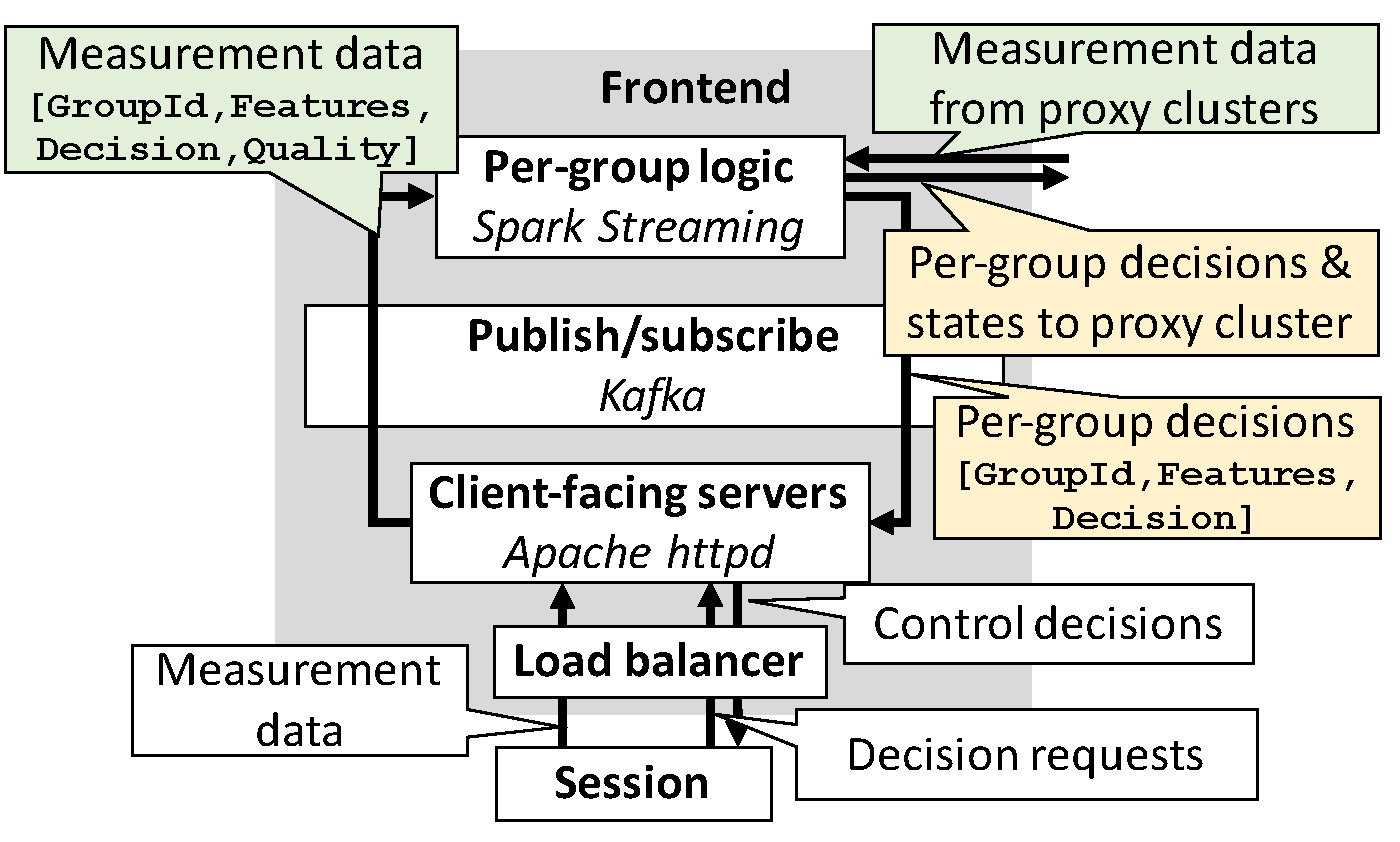
\includegraphics[width=0.6\textwidth]{figures/pytheas-impl-sep-frontend.pdf}
	\label{fig:impl-frontend}
}\\
%\hspace{-0.2cm}
\subfloat[Backend]
{
        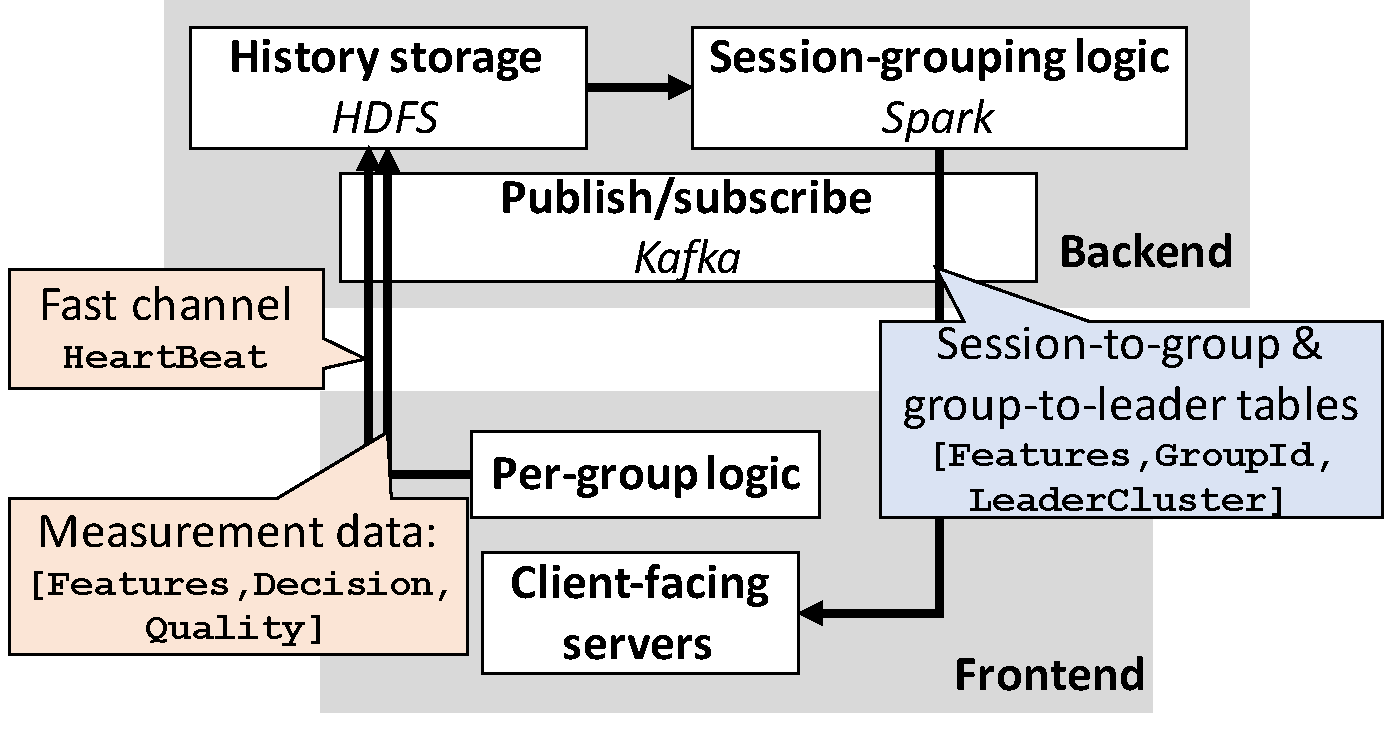
\includegraphics[width=0.6\textwidth]{figures/pytheas-impl-sep-backend.pdf}
	\label{fig:impl-backend}
}
%\hspace{-0.5cm}
%\vspace{-0.2cm}
\caption{Key components and interfaces of \name implementation.}
%\vspace{-0.4cm}
\label{fig:impl-overview}
\end{figure*}


%This section present the key details in implementation, and some lessons we learned in implementing the system.
%Since the key difference between \name and C3 is that the per-group control logic now resides in the frontend cluster (see \Section\ref{sec:system}), we will focus on the implementation of frontend clusters. 
%This section begins with a basic implementation of the two loops of \name, namely per-group control and session grouping,  as described in previous sections.
%We then identify the performance bottlenecks of this basic implementation and how we improved them.
\name is open source ($\approx$ 10K lines of code across Java, python,
and PHP) and can be accessed at~\cite{ddn-source}.  Next, we describe the APIs
for applications to integrate with \name, and then describe the implementation
of frontend and backend, as well as optimizations we used to remove \name's performance
bottlenecks. 

%\tightsubsection{Basic implementation}

\mypara{\name APIs}
Application sessions communicate with \name through two APIs
(Figure~\ref{fig:impl-frontend}): One for requesting control decisions, one for
uploading measurement data.  Both are implemented as standard HTTP POST
messages.  The session features are encoded in
the data field of the POST message.
\name also needs content providers to provide the schema of the message that 
 sessions send to the \name frontend, as well as a list of potential decisions.
Content providers may also provide QoE models that compute QoE metrics from 
the raw quality measurements sent by sessions.

%\vyas{APIs for providers?}

\mypara{Frontend}
Figure~\ref{fig:impl-frontend} shows the key components and interfaces of a
frontend cluster.  When a session sends a control request to \name, the request
will be received by one of the client-facing servers run by Apache
httpd~\cite{httpd}.  The server processes the request with a PHP script, which
first maps the session to a group and its leader cluster by matching
the session features with the session-to-group and group-to-leader tables.
Then the server queries the \mab
logic of the group (Section~\ref{subsec:per-group}), for the most up-to-date
decision of the group, and finally returns the decision to the session.  The
script to process the measurement data uploaded by a session is similar; a
client-facing server maps it to a group, and then forwards it to the per-group
\mab logic. The per-group \mab
logic is a Spark Streaming~\cite{sparkstreaming} program. It maintains a
key-value map (a Spark RDD) between group identification and the per-group \mab states (e.g., most recent decisions),
and updates the states every second by the most recent measurement data in one
MapReduce operation.  
 The communication between these processes is through
Kafka~\cite{kafka}, a distributed publish/subscribe service.  
We used Apache httpd, Spark Streaming, and Kafka, mainly
because they are horizontally scalable and highly resilient to failures of
individual machines.

While the above implementation is functionally sufficient, we observed that 
 the frontend throughput if implemented as-is is low. Next, we discuss 
 the optimizations to overcome the performance bottlenecks.
\begin{itemize}
\item{\em Separating logic from client-facing servers:}
When a client-facing server queries the per-group control logic, the client-facing server is effectively blocked, which significantly reduces the throughput of client-facing servers.
To remove this bottleneck, we add an intermediate process in each client-facing server to decouple querying control logic from responding requests.
It frequently (by default every half second) pulls the fresh decision of each group from per-group logic and writes the decision in a local file of the client-facing server. 
Thus, the client-facing server can find the most up-to-date decisions from local cache without directly querying the control logic.
\item{\em Replacing features with group identifier:}
We found that when the number of session features increases, Spark Streaming has significantly lower throughput as it takes too long to copy the new measurement data from client-facing servers to Kafka and from Kafka to RDDs of Spark Streaming.
This is avoidable, because once the features are mapped to a group by the client-facing servers, the remaining operations (updating and querying per-group logic) are completely feature-agnostic, so we can use group ID as the group identifier and remove all features from messages. 
%This significantly increases the Spark Streaming throughput (see Figure~\ref{fig:eval-optimization-sparkstreaming})
\end{itemize}


\mypara{Backend}
%Session grouping involves both frontend and backend.
Figure~\ref{fig:impl-backend} shows the key components and interfaces of the backend cluster.
Once client-facing servers receive the measurement data from sessions, they will forward the measurement data to the backend cluster.
On receiving these measurement data, the backend stores them in an HDFS for history data, and periodically (by default every 10 minutes) runs the session-grouping logic (Section~\ref{subsec:grouping}) as a Spark~\cite{spark} job to learn the session-group mapping and group-cluster mapping from the stored history data.
These tables are sent to each frontend through Kafka, so that the future messages (requests and measurement data) from sessions will be matched against new tables.
%\cameraremove{To implement the fast channel used for flash crowd detection, each frontend cluster maintains workload statistics and sends them to the backend every 5 seconds. 
%On receiving the data, the backend will then run a simple logic to detect flash crowd (\Section\ref{subsec:flashcrowd}) every 10 seconds.}
In addition, to detect failures of frontend clusters, each frontend cluster sends a small heartbeat message to the backend cluster every 5 seconds.




%\tightsubsection{Performance optimization}
%\label{subsec:optimization}
%
%While this basic implementation offers all functionalities, we found that the frontend throughput could be extremely low.
%This is caused by two bottlenecks which can be alleviated with simple optimization.

%\myparatight{Simplifying session-to-group lookup}
%We used PHP to process requests for its speed and support for runtime edits, but when the number of groups in the session-to-group table becomes too large, this will create a performance bottleneck.
%%Web servers today use scripting languages, such as php, to allow edits at runtime. 
%While this is fine in common cases, we need scripting code to look up a table that could have tens of thousands entries (i.e., groups), and this creates a performance bottleneck.
%In fact, we see throughput drops significantly when the number of groups exceeds certain critical threshold, typically about one thousand.
%We address this bottleneck by dividing all groups into several ``blocks'', so that the number of groups in block is lower than the threshold.
%%, and the total number of blocks is far less than the threshold.
%Each server now first maps a session to a block, and then looks up only the groups in this block.
%As a result, we can achieve the same throughput to a web server without any lookup operation (see Figure~\ref{fig:eval-optimization-throughput-blocklookup}) at little cost on processing time (two lookups instead of one).

%\myparatight{Separating logic from client-facing servers}
%In the basic implementation, to answer each request, the client-facing server needs to query the per-group control logic, during which the client-facing server will be effectively blocked, and significantly increasing the response time of each request.
%To remove this block, we introduce an intermediate process in each client-facing server to split decision updates from request responding.
%It pulls the fresh decision of each group from Kafka on a high frequency (by default every half second), but not on per request base, and writes the decision in a local file. 
%As a result, the client-facing server can return decisions by a simple cache lookup operation, while still preserving the desirable freshness of decisions.
%
%\myparatight{Replacing features with group identifier}
%We found that when we increase the number of session features, Spark Streaming will have significantly lower throughput because it takes too long for Spark Streaming to copy the data out from Kafka and store in memory.
%This is avoidable, because once the features are mapped to a group by the client-facing servers, the rest operations (updating and querying per-group logic) are completely feature-agnostic.
%Thus, once the client-facing servers map feature to a group, we will use group as the identifier and remove features from the message. 
%This significantly increases the Spark Streaming throughput (see Figure~\ref{fig:eval-optimization-sparkstreaming})
%, and also reduce the bandwidth consumption between frontend clusters (Figure~\ref{fig:eval-bandwidth}) (although features have to be sent to the backend for learning critical features and regrouping). 












